
\section{Case Study}
\label{sec:case-study}

\begin{figure}[t]
\centering
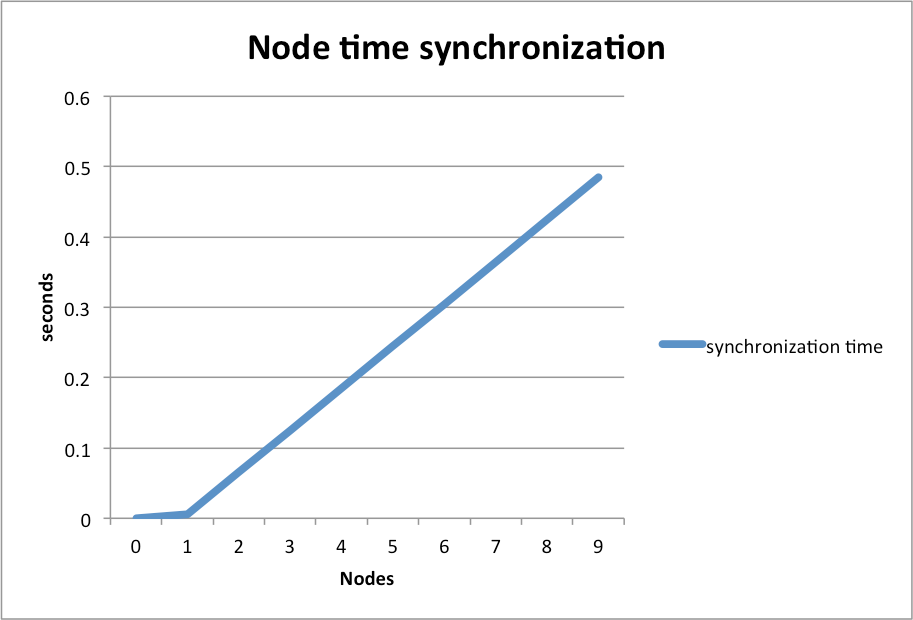
\includegraphics[width=1\columnwidth]{figures/timesynch}
\caption{Time Synchronization performance evaluation.}
\label{fig:timeCorrection}
\end{figure}

Our main goal is to verify how different schedules impact on the performance of a network. In particular we focused on two metrics. The first one is the time of first synchronization of each node in the network. This metric gives us an idea of how \emph{reactive} is the network. The second metric is the power consumption of each node in the network for a specific period of time. 

\subsection{Experiment Configuration}
\label{sec:exp_config}

In all the experiments, nodes are organized to form a chain topology. With this topology, each node can communicate only with the two neighbors that are closer to it. To realize this short-distance communication, we use the Ptolemy \emph{Wireless Director} with a \emph{limited range} channel model.
We consider three different schedules. The first one, which has a 4 timeslots period \footnote{Each timeslot has a duration of 15ms}, is \{\texttt{ADV}, \texttt{TX}, \texttt{RX}, \texttt{OFF}\}, following the follo

%%% Local Variables: 
%%% mode: latex
%%% TeX-master: "ee219d"
%%% End: 
